% Appendix Template

\chapter{Empirical Distance Matrices} % Main appendix title

\label{AppendixC} % Change X to a consecutive letter; for referencing this appendix elsewhere, use \ref{AppendixX}

\lhead{Appendix C. \emph{Empirical Distance Matrices}} % Change X to a consecutive letter; this is for the header on each page - perhaps a shortened title

The distance matrix $d_{ij}$ is one of the ingredient parameters of the FHN network model. It is used to quantify the time delays $\Delta t_{ij}$ between nodes $i$ and $j$, i.e. $\Delta t_{ij} = d_{ij} / v$, where $v$ is the signal propagation velocity along the axons \citep{VUK13, GHO08a}. The neuronal time-series of functionally and anatomically derived adjacency matrices is extracted  by using different $d_{ij}$ data. For the FCM, $d_{ij}$ is the matrix of Euclidean distances between centers of brain regions from which BOLD time series are extracted \citep{KAI06}. For the ACM, $d_{ij}$ is empirically provided with together with anatomical connectivity map \citep{ITU08}. 



\begin{figure}[htbp]
 
  \centering
	 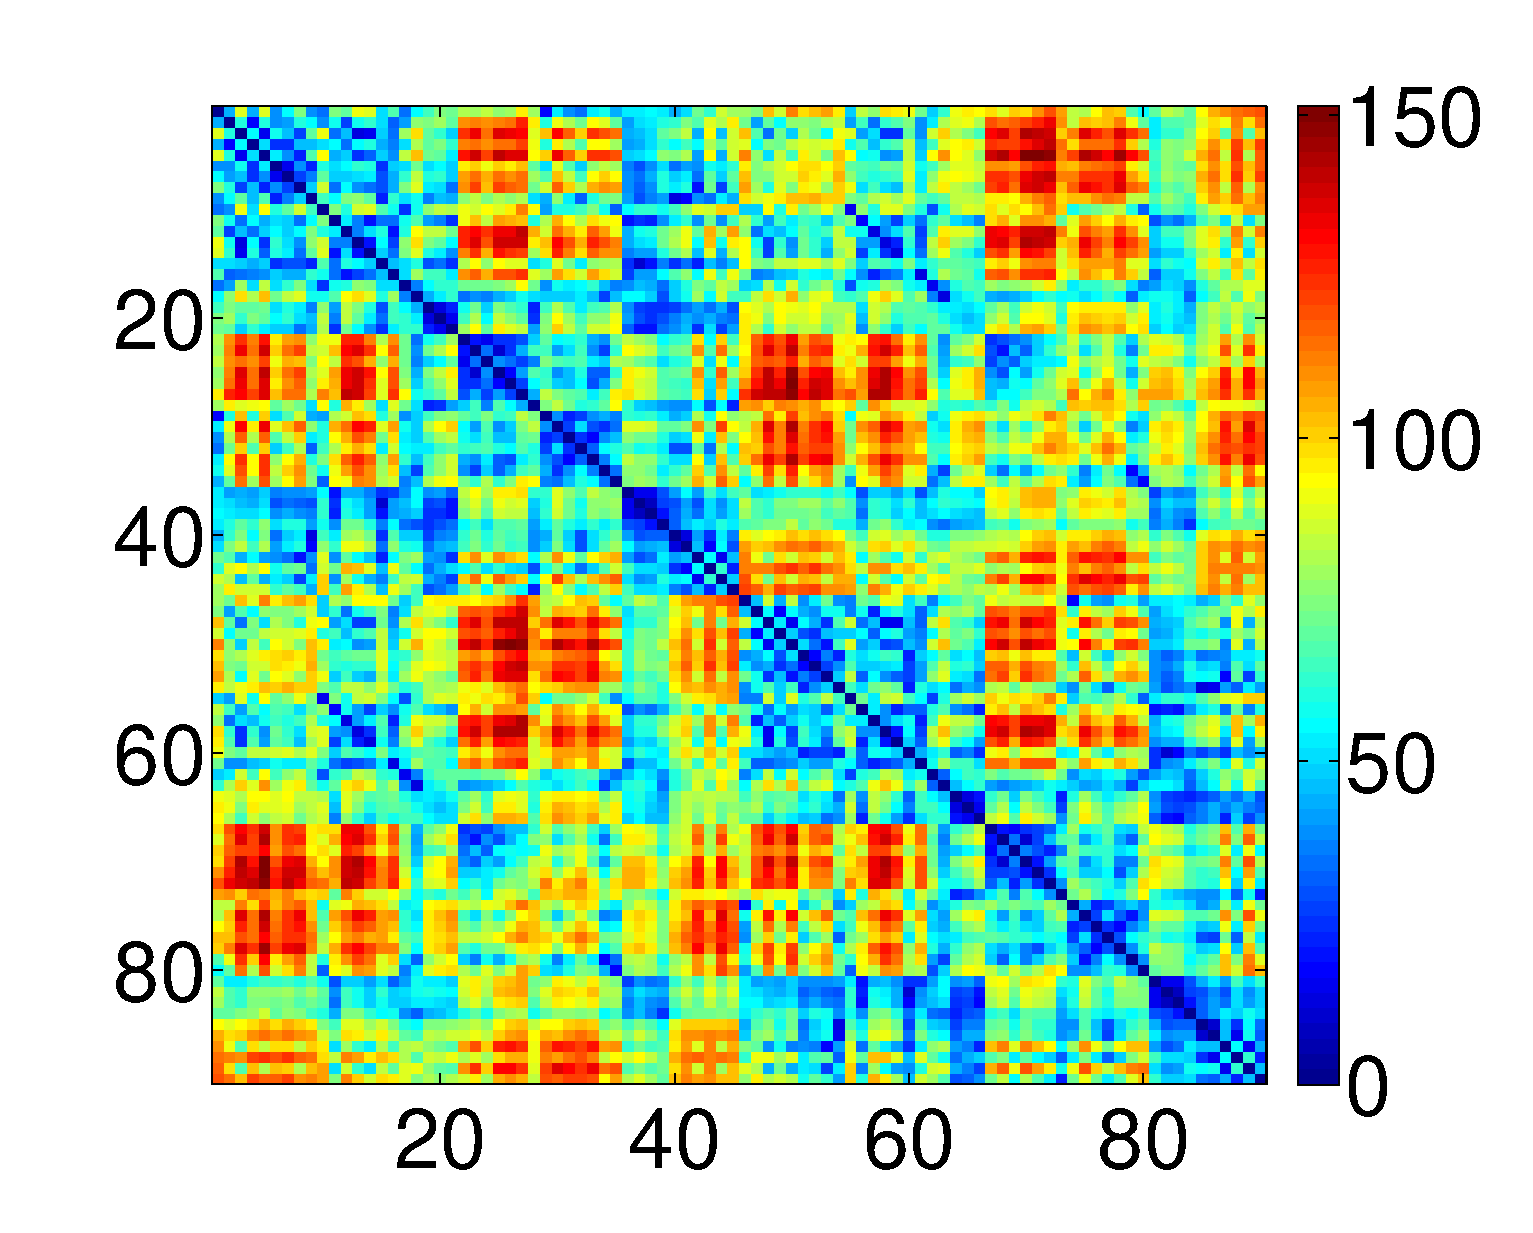
\includegraphics[width=0.49\textwidth]{Figures/distance_FCM.eps}
	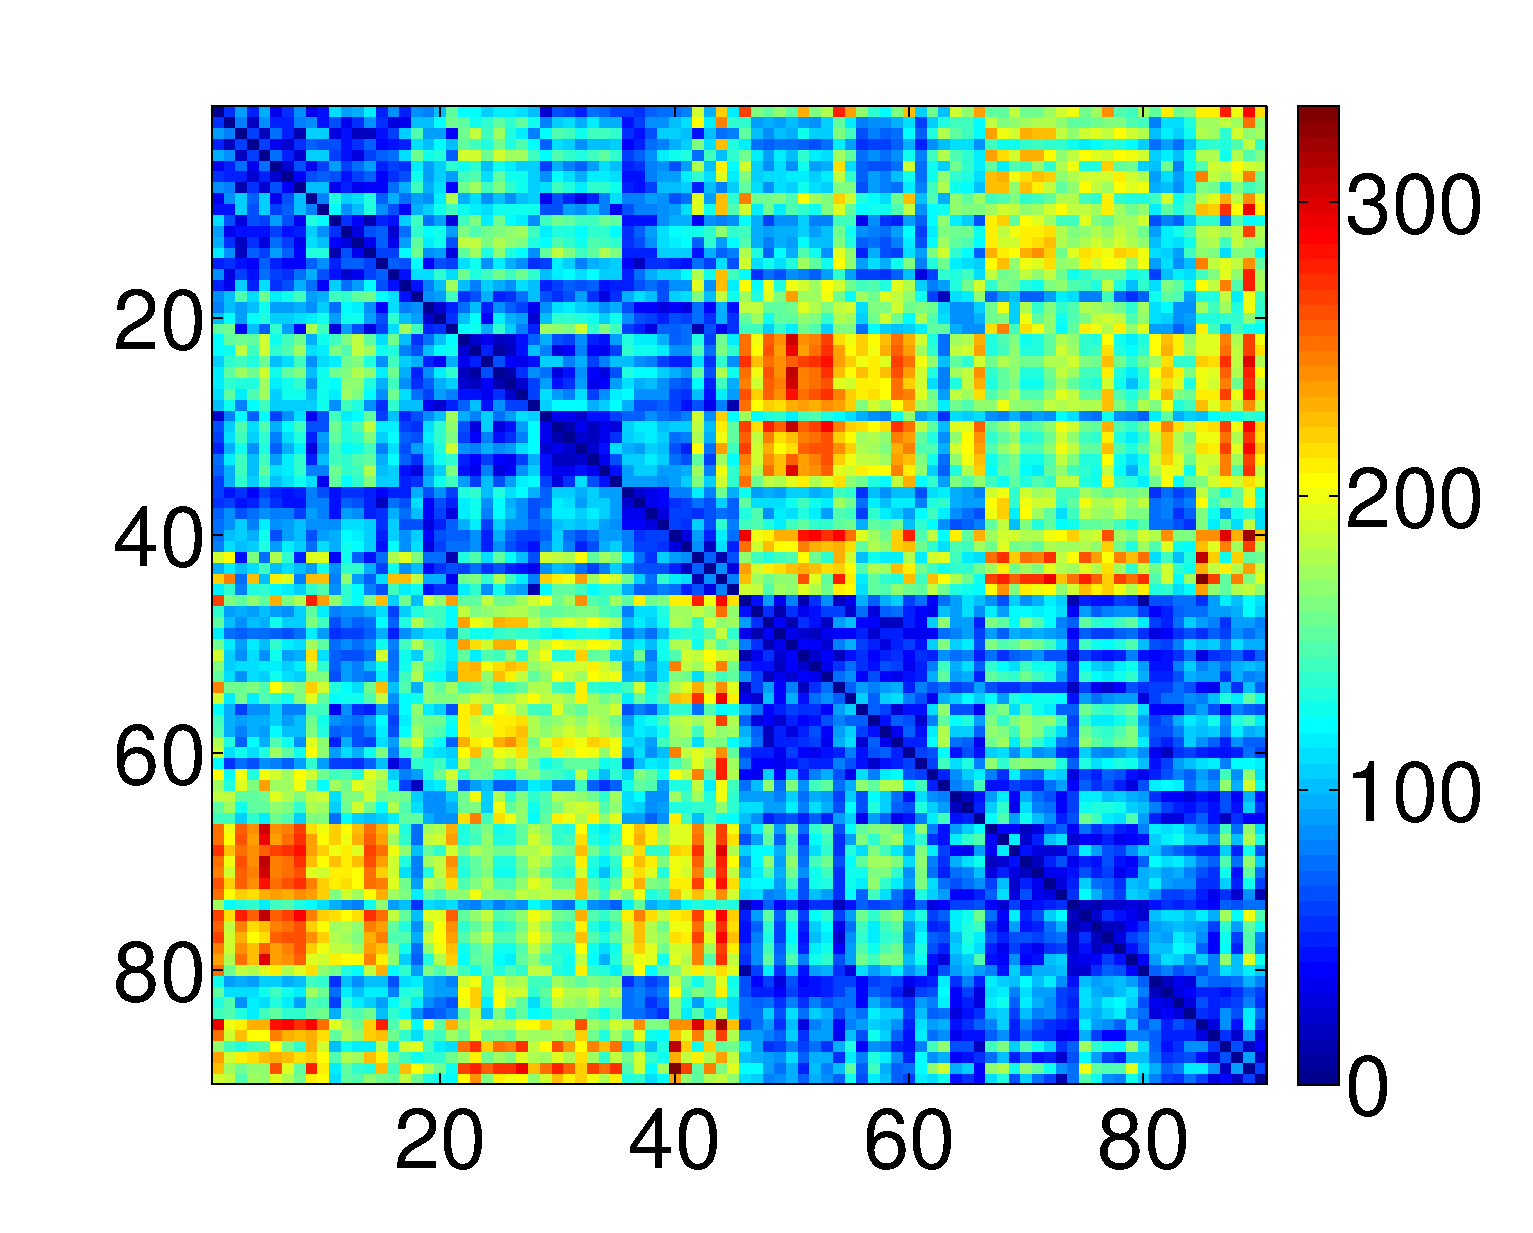
\includegraphics[width=0.49\textwidth]{Figures/distance_ACM.eps}		
	\rule{35em}{0.5pt}  
  \caption[Distance Matrices]{$d_{ij}$ of the functional connectivity map (left) and anatomical connectivity map (left). The colorbars are in units of mm.} 
    \label{fig:Distance Matrices}
 	
\end{figure}
